\section{ICMP Echo Response}
The ICMP Echo Response Packet processing module receives and generates
responses to the traditional ping network diagnostic tool. Upon
reception of an echo-request it will generate an echo-response back to
the sender, including any of the data that the sender sent in its
payload.

\subsection{Implementation}
\begin{figure}
\begin{centering}
\includegraphics[scale=0.8]{ping.svg}
\end{centering}
\caption{ICMP Echo response packet processing module}
\label{ping}
\end{figure}

\begin{figure}
\begin{centering}
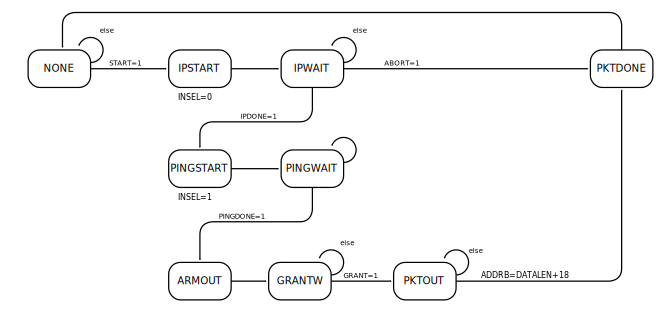
\includegraphics[scale=0.8]{ping.fsm.svg}
\end{centering}
\caption{ICMP Echo response packet processing module FSM}
\label{ping.fsm}
\end{figure}

\begin{figure}
\begin{centering}
\includegraphics[scale=0.8]{ping.ip.svg}
\end{centering}
\caption{ICMP Echo response packet processing module}
\label{ping.ip}
\end{figure}

\begin{figure}
\begin{centering}
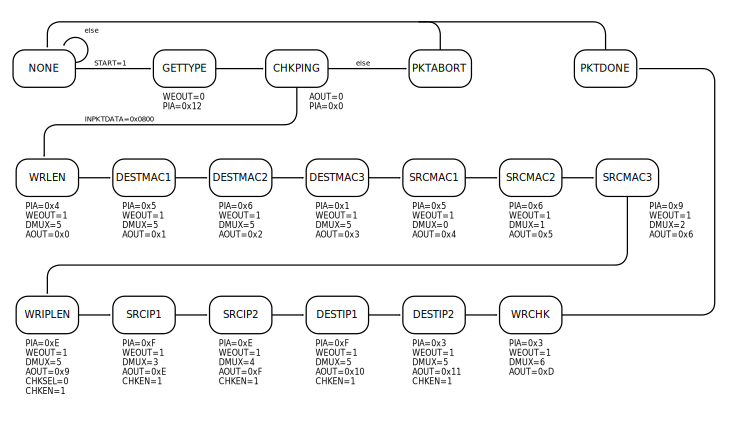
\includegraphics[scale=0.8]{ping.ip.fsm.svg}
\end{centering}
\caption{ICMP Echo response packet processing module FSM}
\label{ping.ip.fsm}
\end{figure}


\begin{figure}
\begin{centering}
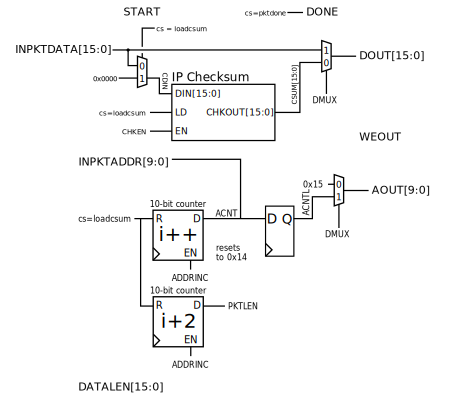
\includegraphics[scale=0.8]{ping.icmp.svg}
\end{centering}
\caption{ICMP Echo response packet processing module}
\label{ping}
\end{figure}

\begin{figure}
\begin{centering}
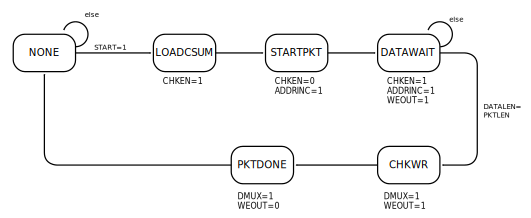
\includegraphics[scale=0.8]{ping.icmp.fsm.svg}
\end{centering}
\caption{ICMP Echo response packet processing module FSM}
\label{ping.fsm}
\end{figure}

The module has two primary components, an IP Writer (which writes
frame, MAC, and IP header information) and an ICMP Writer, which
writes the relevant ICMP header information as well as copying the
ping body data contents into the output buffer.

These two components are given multiplexed access to the output
buffer; once both have had a chance to write their data, the main FSM
outputs the packet via the TX Mux.

The design of both components is similar to the UDPHeaderWriter module. 
